
\chapter{使用简介}
\label{chap:guide}

为方便使用及更好的展示~\LaTeX{}~排版的优秀特性,本人对模板的框架和文件体系进行了细致地处理,尽可能地对各个功能和板块进行了模块化和封装,对于初学者来说,众多的文件目录也许会让人觉得有些无所适从,但阅读完下面的使用说明后,您会发现原来使用思路是简单而清晰的,而且,当对~\LaTeX{}~ 有一定的认识和了解后,会发现其相对~Word~类排版系统的极具吸引力的优秀特性。所以,如果您是初学者,请不要退缩,请稍加尝试和坚持,让自己领略到~\LaTeX{}~的非凡魅力。 并可以通过阅读相关资料如~ \citep{wikibook2014latex}~ 来完善自己的使用知识。

\section{先试试效果}

ucasthesis~模板不仅只是提供了相应的类文件,同时也提供了包括参考文献等在内的完成学位论文的一切要素,所以,下载时,推荐下载整个~ucasthesis~文件夹,而不是单独的文档类。

下载~ucasthesis~文件夹并解压后,请在文件夹内找到~“Compile.bat”,双击运行,即可获得本说明文档,而这,也完成了学习使用此模板撰写论文的一半进程,什么?这就学成一半了,这么简单???,是的,就这么简单!

编译完成后,可以进入各个子目录逛逛,熟悉下模板框架。

\section{常见使用问题}

\begin{enumerate}
  \item 模板文档的编码为~utf-8~编码,若出现文本编辑器无法打开文档或打开文档乱码的问题,请检查您使用的编辑器对utf-8编码的支持,如果使用~WinEdit~作为文本编辑器,应在其

  “options --》 Preferences --》 wrapping”

  选项卡下将两种 “Wrapping Modes” 中的内容:

  “TeX;HTML;ANSI;ASCII|DTX...”

  修改为:

  “TeX;\textbf{UTF-8|ACP;}HTML;ANSI;ASCII|DTX...”

  同时,取消

  “options --》 Preferences --》 Unicode”

  中的“Enable ANSI Format...”选项。
\end{enumerate}

\section{各文档及目录简介}

\subsection{Thesis.tex文档 }

Thesis.tex文档为主文档,其设计和规划了论文的整体框架,通过对其的阅读可以让用户了解整个论文框架的搭建。

\subsection{Compile.bat}

Compile.bat为编译此模板的Dos脚本,通过双击运行此脚本即可获得编译后的PDF文档,编译生成的文档及临时文件皆位于Tmp文件夹内。在此脚本中可以设定编译器为“pdflatex” or “xelatex” (default,且极力推荐使用xelatex 编译中文及中英文混排的\LaTeX{}文档)。

若你倾向于使用WinEdit的编译方式,则请在 "Thesis.tex" 和 "Main\textunderscore Content.tex" 中为所有文件提供完整的搜索路径。 如 

\verb+\chapter{中国科学院大学学位论文撰写要求}

学位论文是研究生科研工作成果的集中体现,是评判学位申请者学术水平、授予其学位的主要依据,是科研领域重要的文献资料。根据《科学技术报告、学位论文和学术论文的编写格式》(GB/T 7713-1987)、《学位论文编写规则》(GB/T 7713.1-2006)和《文后参考文献著录规则》(GB7714—87)等国家有关标准,结合中国科学院大学(以下简称“国科大”)的实际情况,特制订本规定。

\section{论文无附录者无需附录部分}

\section{测试公式编号 \texorpdfstring{$\Lambda,\lambda,\theta,\bar{\Lambda},\sqrt{S_{NN}}$}{$\textLambda,\textlambda,\texttheta,\bar{\textLambda},\sqrt{S_{NN}}$}} \label{sec:testmath}

\begin{equation} \label{eq:appedns}
    \adddotsbeforeeqnnum%
    \begin{cases}
        \frac{\partial \rho}{\partial t} + \nabla\cdot(\rho\Vector{V}) = 0\\
        \frac{\partial (\rho\Vector{V})}{\partial t} + \nabla\cdot(\rho\Vector{V}\Vector{V}) = \nabla\cdot\Tensor{\sigma}\\
        \frac{\partial (\rho E)}{\partial t} + \nabla\cdot(\rho E\Vector{V}) = \nabla\cdot(k\nabla T) + \nabla\cdot(\Tensor{\sigma}\cdot\Vector{V})
    \end{cases}
\end{equation}
\begin{equation}
    \adddotsbeforeeqnnum%
    \frac{\partial }{\partial t}\int\limits_{\Omega} u \, \mathrm{d}\Omega + \int\limits_{S} \unitVector{n}\cdot(u\Vector{V}) \, \mathrm{d}S = \dot{\phi}
\end{equation}
\[
    \begin{split}
        \mathcal{L} \{f\}(s) &= \int _{0^{-}}^{\infty} f(t) e^{-st} \, \mathrm{d}t, \ 
        \mathscr{L} \{f\}(s) = \int _{0^{-}}^{\infty} f(t) e^{-st} \, \mathrm{d}t\\
        \mathcal{F} {\bigl (} f(x+x_{0}) {\bigr )} &= \mathcal{F} {\bigl (} f(x) {\bigr )} e^{2\pi i\xi x_{0}}, \ 
        \mathscr{F} {\bigl (} f(x+x_{0}) {\bigr )} = \mathscr{F} {\bigl (} f(x) {\bigr )} e^{2\pi i\xi x_{0}}
    \end{split}
\]

mathtext: $A,F,L,2,3,5,\sigma$, mathnormal: $A,F,L,2,3,5,\sigma$, mathrm: $\mathrm{A,F,L,2,3,5,\sigma}$.

mathbf: $\mathbf{A,F,L,2,3,5,\sigma}$, mathit: $\mathit{A,F,L,2,3,5,\sigma}$, mathsf: $\mathsf{A,F,L,2,3,5,\sigma}$.

mathtt: $\mathtt{A,F,L,2,3,5,\sigma}$, mathfrak: $\mathfrak{A,F,L,2,3,5,\sigma}$, mathbb: $\mathbb{A,F,L,2,3,5,\sigma}$.

mathcal: $\mathcal{A,F,L,2,3,5,\sigma}$, mathscr: $\mathscr{A,F,L,2,3,5,\sigma}$, boldsymbol: $\boldsymbol{A,F,L,2,3,5,\sigma}$.

\section{测试生僻字}

霜蟾盥薇曜灵霜颸妙鬘虚霩淩澌菀枯菡萏泬寥窅冥毰毸濩落霅霅便嬛岧峣瀺灂姽婳愔嫕飒纚棽俪緸冤莩甲摛藻卮言倥侗椒觞期颐夜阑彬蔚倥偬澄廓簪缨陟遐迤逦缥缃鹣鲽憯懔闺闼璀错媕婀噌吰澒洞阛闠覼缕玓瓑逡巡諓諓琭琭瀌瀌踽踽叆叇氤氲瓠犀流眄蹀躞赟嬛茕頔璎珞螓首蘅皋惏悷缱绻昶皴皱颟顸愀然菡萏卑陬纯懿犇麤掱暒 墌墍墎墏墐墒墒墓墔墕墖墘墖墚墛坠墝增墠墡墢墣墤墥墦墧墨墩墪樽墬墭堕墯墰墱墲坟墴墵垯墷墸墹墺墙墼墽垦墿壀壁壂壃壄壅壆坛壈壉壊垱壌壍埙壏壐壑壒压壔壕壖壗垒圹垆壛壜壝垄壠壡坜壣壤壥壦壧壨坝塆圭嫶嫷嫸嫹嫺娴嫼嫽嫾婳妫嬁嬂嬃嬄嬅嬆嬇娆嬉嬊娇嬍嬎嬏嬐嬑嬒嬓嬔嬕嬖嬗嬘嫱嬚嬛嬜嬞嬟嬠嫒嬢嬣嬥嬦嬧嬨嬩嫔嬫嬬奶嬬嬮嬯婴嬱嬲嬳嬴嬵嬶嬷婶嬹嬺嬻嬼嬽嬾嬿孀孁孂娘孄孅孆孇孆孈孉孊娈孋孊孍孎孏嫫婿媚嵭嵮嵯嵰嵱嵲嵳嵴嵵嵶嵷嵸嵹嵺嵻嵼嵽嵾嵿嶀嵝嶂嶃崭嶅嶆岖嶈嶉嶊嶋嶌嶍嶎嶏嶐嶑嶒嶓嵚嶕嶖嶘嶙嶚嶛嶜嶝嶞嶟峤嶡峣嶣嶤嶥嶦峄峃嶩嶪嶫嶬嶭崄嶯嶰嶱嶲嶳岙嶵嶶嶷嵘嶹岭嶻屿岳帋巀巁巂巃巄巅巆巇巈巉巊岿巌巍巎巏巐巑峦巓巅巕岩巗巘巙巚帠帡帢帣帤帨帩帪帬帯帰帱帲帴帵帷帹帺帻帼帽帾帿幁幂帏幄幅幆幇幈幉幊幋幌幍幎幏幐幑幒幓幖幙幚幛幜幝幞帜幠幡幢幤幥幦幧幨幩幪幭幮幯幰幱庍庎庑庖庘庛庝庠庡庢庣庤庥庨庩庪庬庮庯庰庱庲庳庴庵庹庺庻庼庽庿廀厕廃厩廅廆廇廋廌廍庼廏廐廑廒廔廕廖廗廘廙廛廜廞庑廤廥廦廧廨廭廮廯廰痈廲廵廸廹廻廼廽廿弁弅弆弇弉弖弙弚弜弝弞弡弢弣弤弨弩弪弫弬弭弮弰弲弪弴弶弸弻弼弽弿彖彗彘彚彛彜彝彞彟彴彵彶彷彸役彺彻彽彾佛徂徃徆徇徉后徍徎徏径徒従徔徕徖徙徚徛徜徝从徟徕御徢徣徤徥徦徧徨复循徫旁徭微徯徰徱徲徳徴徵徶德徸彻徺忁忂惔愔忇忈忉忔忕忖忚忛応忝忞忟忪挣挦挧挨挩挪挫挬挭挮挰掇授掉掊掋掍掎掐掑排掓掔掕挜掚挂掜掝掞掟掠采探掣掤掦措掫掬掭掮掯掰掱掲掳掴掵掶掸掹掺掻掼掽掾掿拣揁揂揃揅揄揆揇揈揉揊揋揌揍揎揑揓揔揕揖揗揘揙揤揥揦揧揨揫捂揰揱揲揳援揵揶揷揸揻揼揾揿搀搁搂搃搄搅搇搈搉搊搋搌搎搏搐搑搒摓摔摕摖摗摙摚摛掼摝摞摠摡斫斩斮斱斲斳斴斵斶斸旪旫旮旯晒晓晔晕晖晗晘晙晛晜晞晟晠晡晰晣晤晥晦晧晪晫晬晭晰晱晲晳晴晵晷晸晹晻晼晽晾晿暀暁暂暃暄暅暆暇晕晖暊暋暌暍暎暏暐暑暒暓暔暕暖暗旸暙暚暛暜暝暞暟暠暡暣暤暥暦暧暨暩暪暬暭暮暯暰昵暲暳暴暵暶暷暸暹暺暻暼暽暾暿曀曁曂曃晔曅曈曊曋曌曍曎曏曐曑曒曓曔曕曗曘曙曚曛曜曝曞曟旷曡曢曣曤曥曦曧昽曩曪曫晒曭曮曯椗椘椙椚椛検椝椞椟椠椡椢椣椤椥椦椧椨椩椪椫椬椭椮。
+ 

应改为 

\verb+\input{./Tex/Appeddix}+。

\subsection{Tmp文件夹}

运行编译脚本Compile.bat后,编译所生成的文档皆存于Tmp文件夹内,包括编译得到的pdf文档,其存在是为了保持工作空间的整洁,因为好的心情是很重要的.

\subsection{Style文件夹}

Style文件夹内包含有ucasthesis文档类的定义文件和配置文件,对于有特殊需求的用户,通过对它们的修改可以实现特定的类设定。

\begin{enumerate}
  \item ucasthesis.cls: 文档类定义文件,论文的最核心的格式即通过它来定义的。
  \item ucasthesis.cfg: 文档类配置文件,通过它设定论文的某些项目的显示内容,如“abstract”显示为“摘要”,“table of content”显示为“目~~~~录”而不是“目录”等(如果愿意,你也可以改过来)。
  \item commons.sty: 一些常用的文档设定, 如参考文献样式和文献引用样式等。
  \item custom.sty: 用户自定义命令的放置位置以及用来实现一些个性化设定,
\end{enumerate}

\subsection{Tex文件夹}

Tex文件夹内为论文的所有实体内容,正常情况下,这也是你\textbf{使用此模板撰写学文论文时,主要关注和修改的一个位置},详细分类介绍如下:

\begin{itemize}
  \item Frontpage.tex: 为论文封面内容, 及中英文摘要。
  \item Main\textunderscore Content.tex: 对需要出现的Chapter进行索引,开始写论文时,可以只索引当前章节,以便快速编译和查看,当最终所有章节完成后,再对所有章节进行索引即可。
  \item Chap\textunderscore XXXXX.tex: 为论文主体的各个章节,用户可根据需要添加和撰写,最终需要包含在论文中的章节,须在Main\textunderscore Content.tex中进行索引。
  \item Appendix.tex: 为附录内容
  \item Backmatter.tex: 为发表文章信息,致谢部分等。
\end{itemize}

\subsection{Img文件夹}

Img文件夹用于放置论文中所需要的图类文件,支持格式有:.jpg, .png, .pdf。其中,ucas.jpg为国科大校徽。

\subsection{Biblio文件夹}

Biblio文件夹内放置参考文献的索引信息文件:Myrefs.bib,此文件包含了需要引用的参考文献信息。

\section{数学公式、图片插入、参考文献等功能}

\subsection{数学公式}

常用数学公式的命令代码模板,请见如下WiKi:\url{http://zh.wikipedia.org/wiki/Help:%E6%95%B0%E5%AD%A6%E5%85%AC%E5%BC%8F}

\subsection{图片插入}

论文中图片的插入通常分为单图和多图,下面分别加以介绍:

单图插入:假设插入名为“ITC\textunderscore Q\textunderscore Criteria”(后缀可以为.jpg、.png、.pdf,下同)的图片,其效果如图\ref{fig:ITC_Q_Criteria},其命令可为:
\begin{verbatim}
\begin{figure}[!htbp]
  \centering
  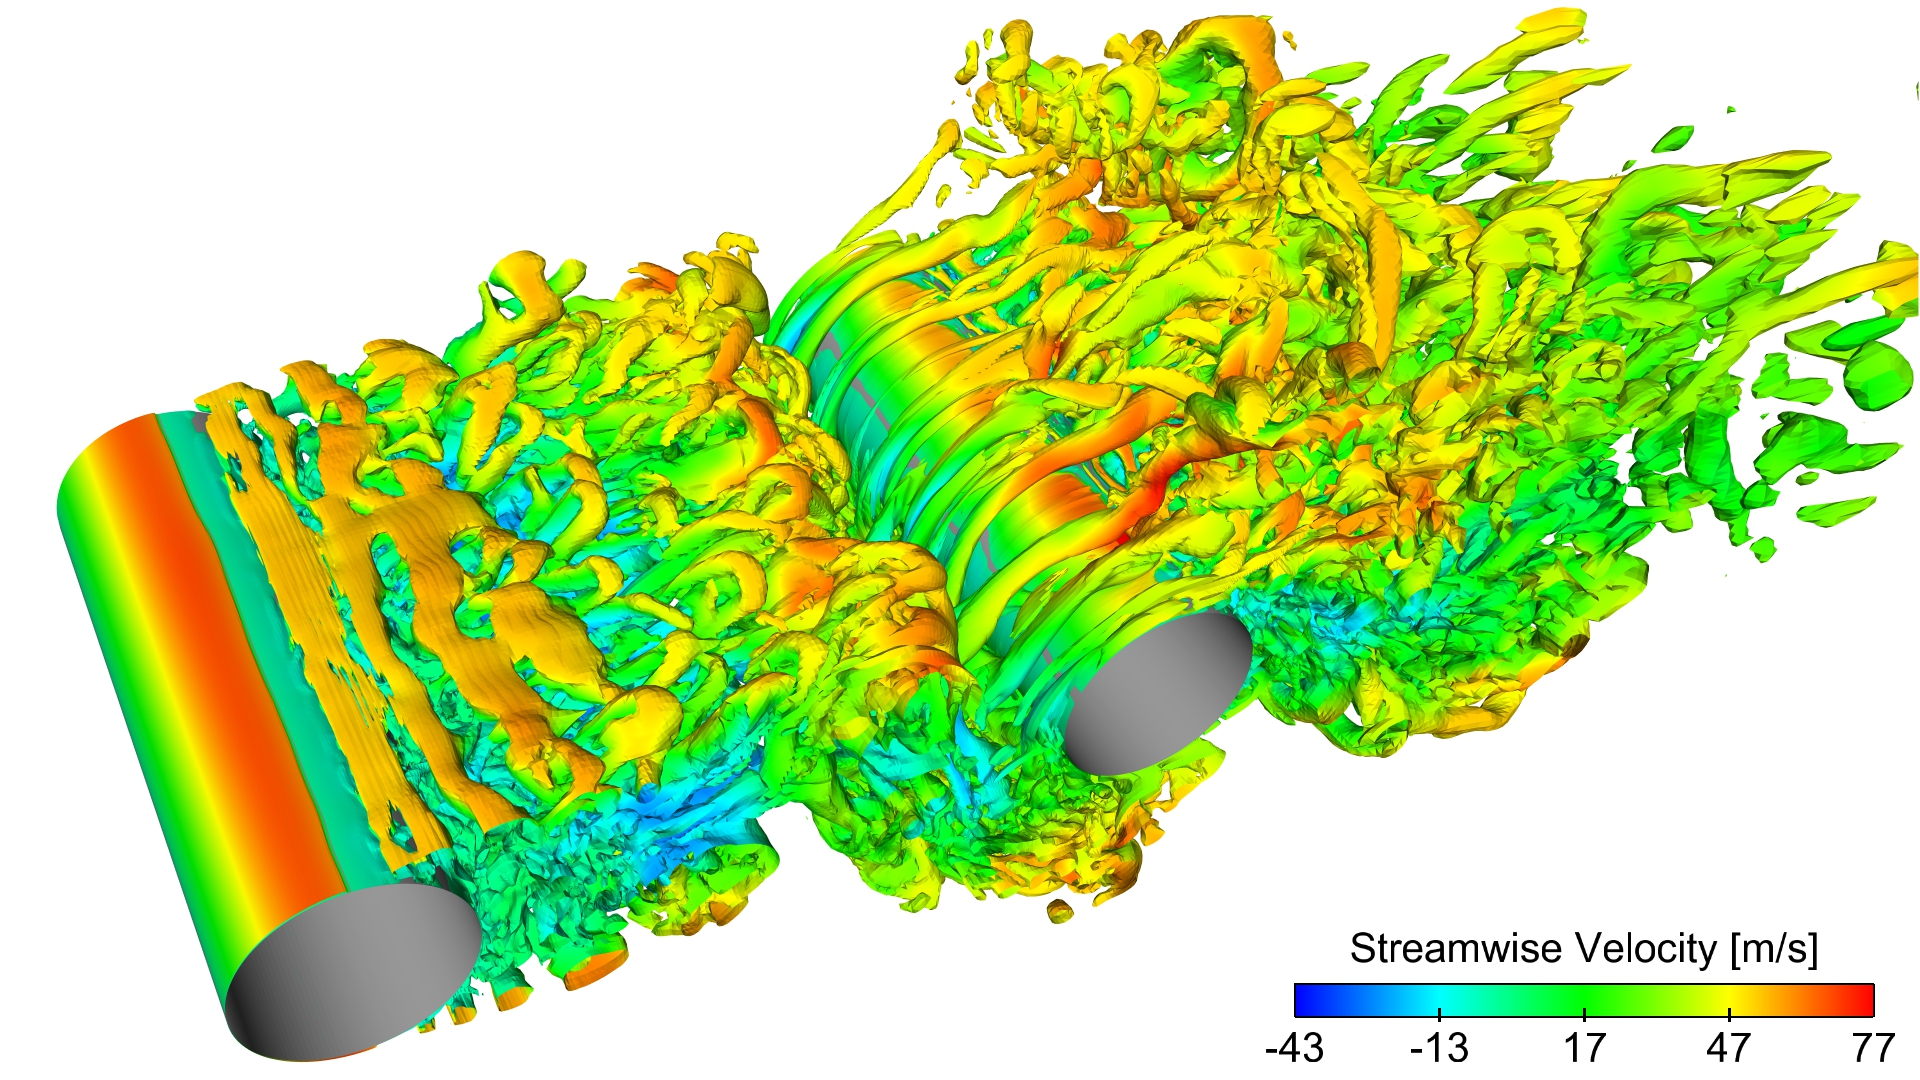
\includegraphics[width=\MyFactor\textwidth]{ITC_Q_Criteria}
  \caption{Q判据等值面图}
  \label{fig:ITC_Q_Criteria}
\end{figure}
\end{verbatim}
\begin{figure}[!htbp]
  \centering
  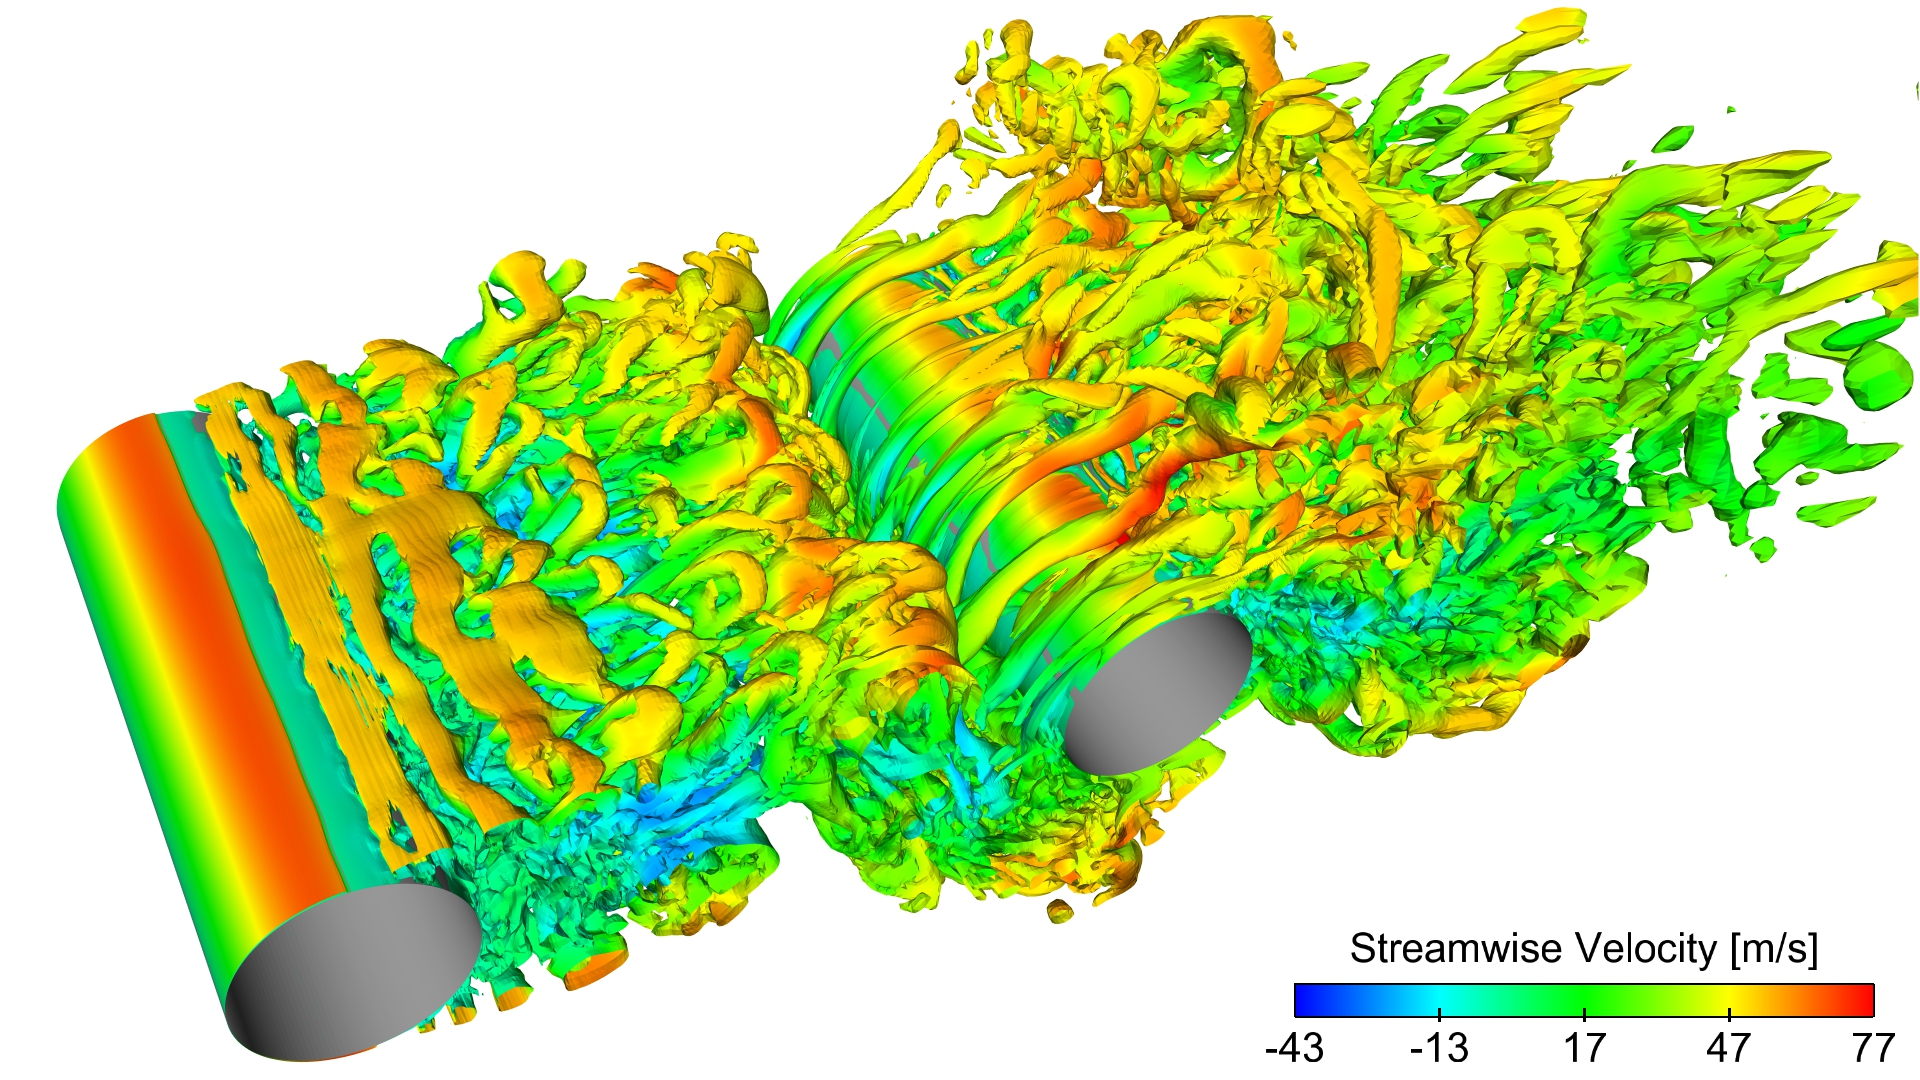
\includegraphics[width=\MyFactor\textwidth]{ITC_Q_Criteria}
  \caption{Q判据等值面图}
  \label{fig:ITC_Q_Criteria}
\end{figure}

如果插图的上下空白区域过大,希望减少插入图片后的留白,以图片“Y”为例(图\ref{fig:Y}),可以使用如下代码模板:
\begin{verbatim}
\begin{figure}[!htbp]
  \centering
  %trim option's parameter order: left bottom right top
  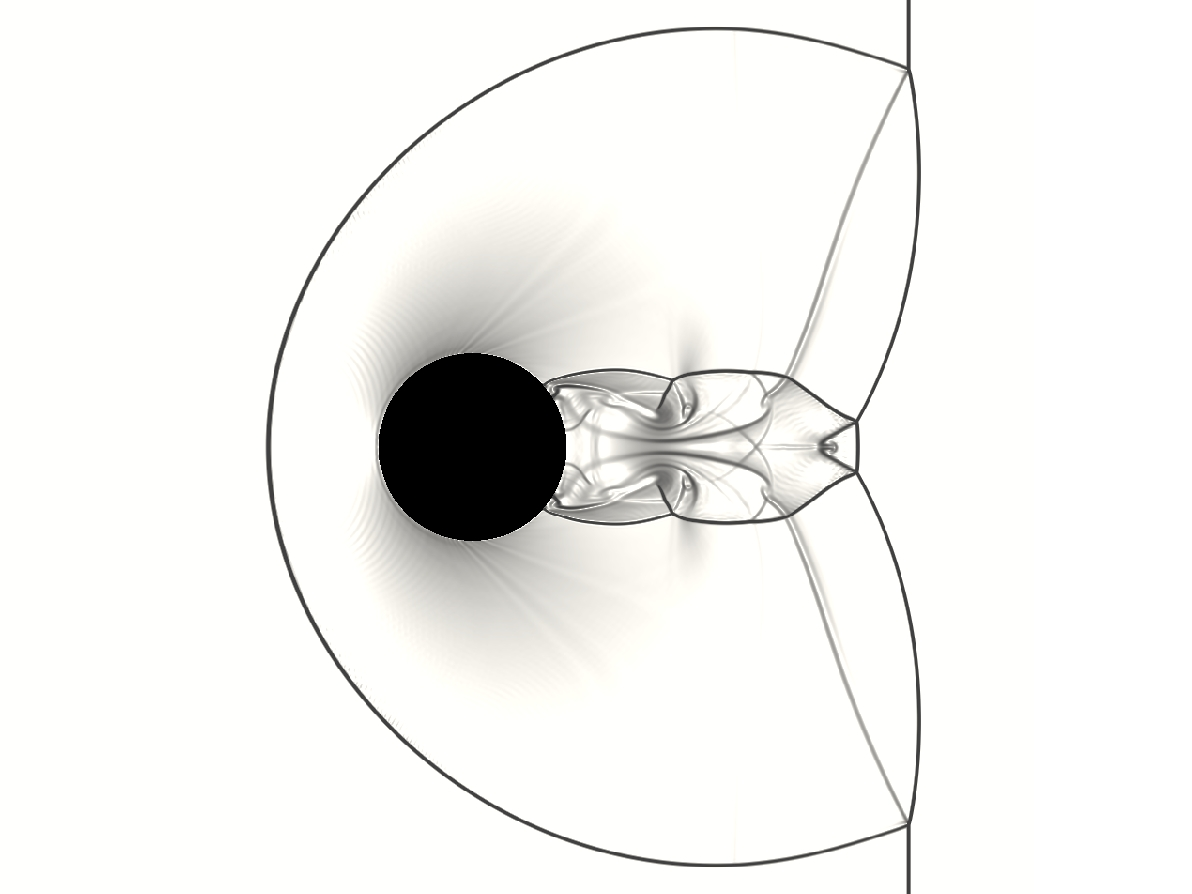
\includegraphics[trim = 0mm 25mm 0mm 30mm, clip, width=\MyFactor\textwidth]{Y}
  \caption{Tandem cylinder clip view}
  \label{fig:Y}
\end{figure}
\end{verbatim}
\begin{figure}[!htbp]
  \centering
  %trim option's parameter order: left bottom right top
  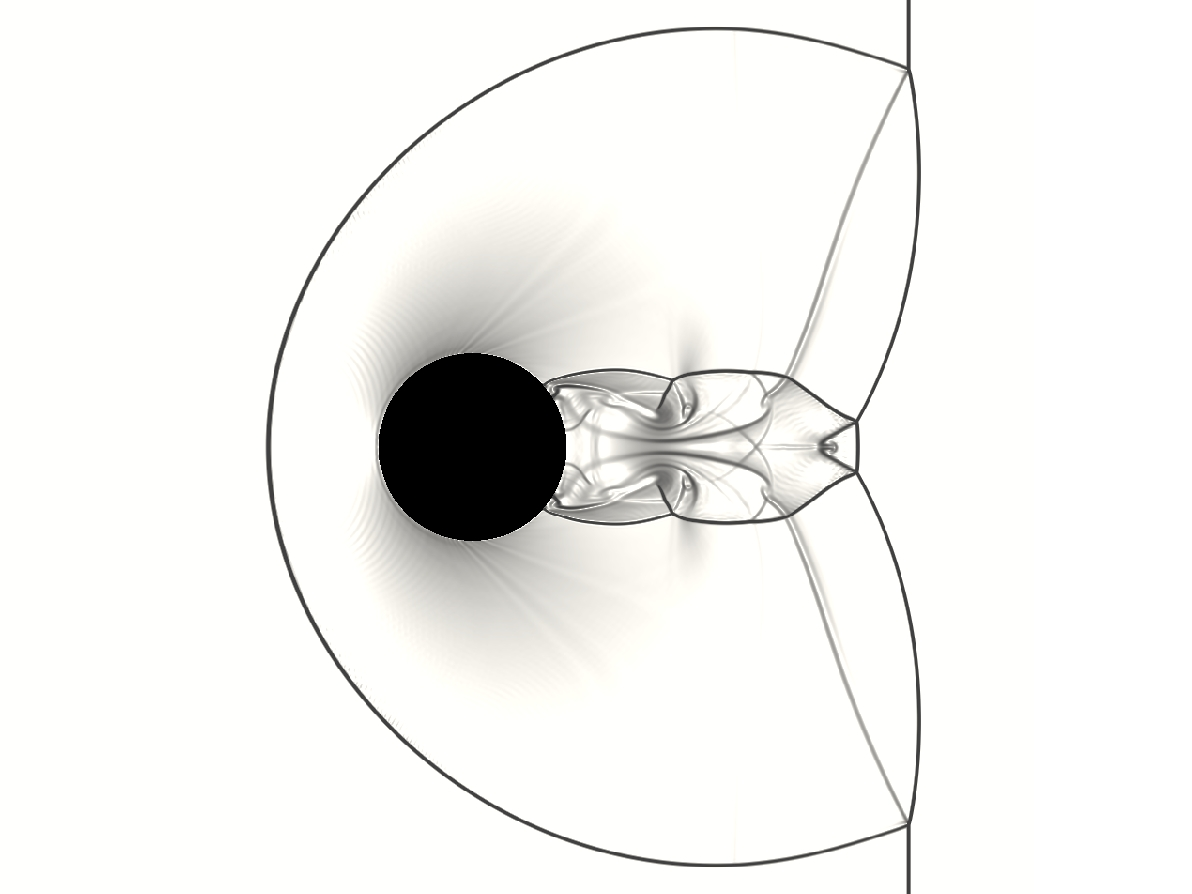
\includegraphics[trim = 0mm 25mm 0mm 30mm, clip, width=\MyFactor\textwidth]{Y}
  \caption{Tandem cylinder clip view}
  \label{fig:Y}
\end{figure}

多图的插入如图\ref{fig:HC_OASPL},其代码如下,其中,\verb|\MyFactor|和\verb|\MySubFactor|是在“custom.sty”中定义的两个小数,用于全局控制插入图片的宽度,用户可以适当调整其数值,或者直接在命令调用时,用需要的小数值替代它们就行。
\begin{verbatim}
\begin{figure}[!htbp]
  \centering
  \begin{subfigure}[b]{\MySubFactor\textwidth}
    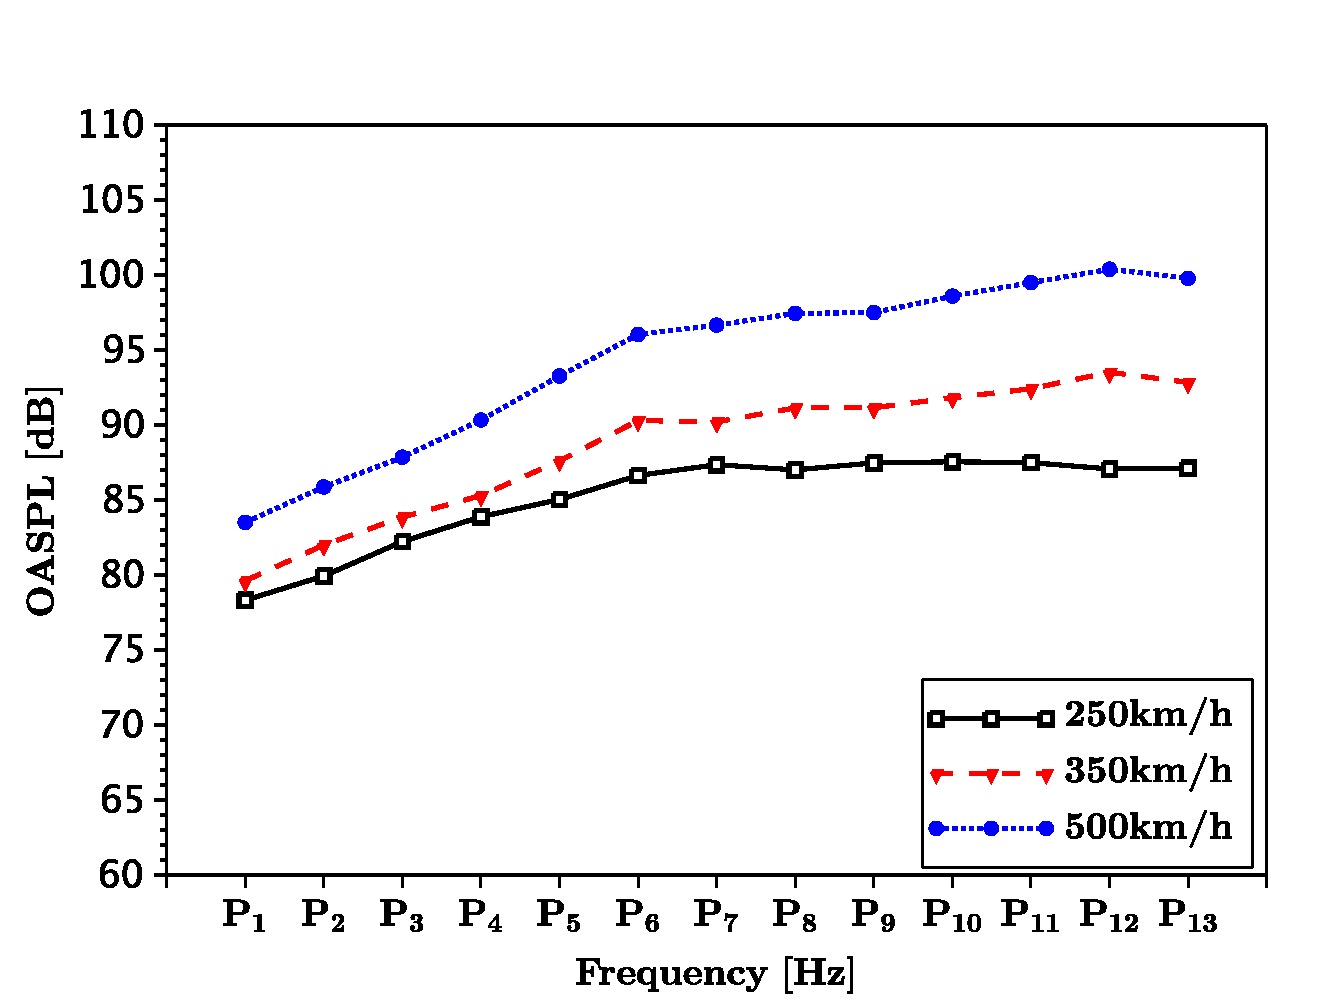
\includegraphics[width=\textwidth]{HC_OASPL_A}
    \caption{}
    \label{fig:HC_OASPL_A}
  \end{subfigure}%
  ~%add desired spacing
  \begin{subfigure}[b]{\MySubFactor\textwidth}
    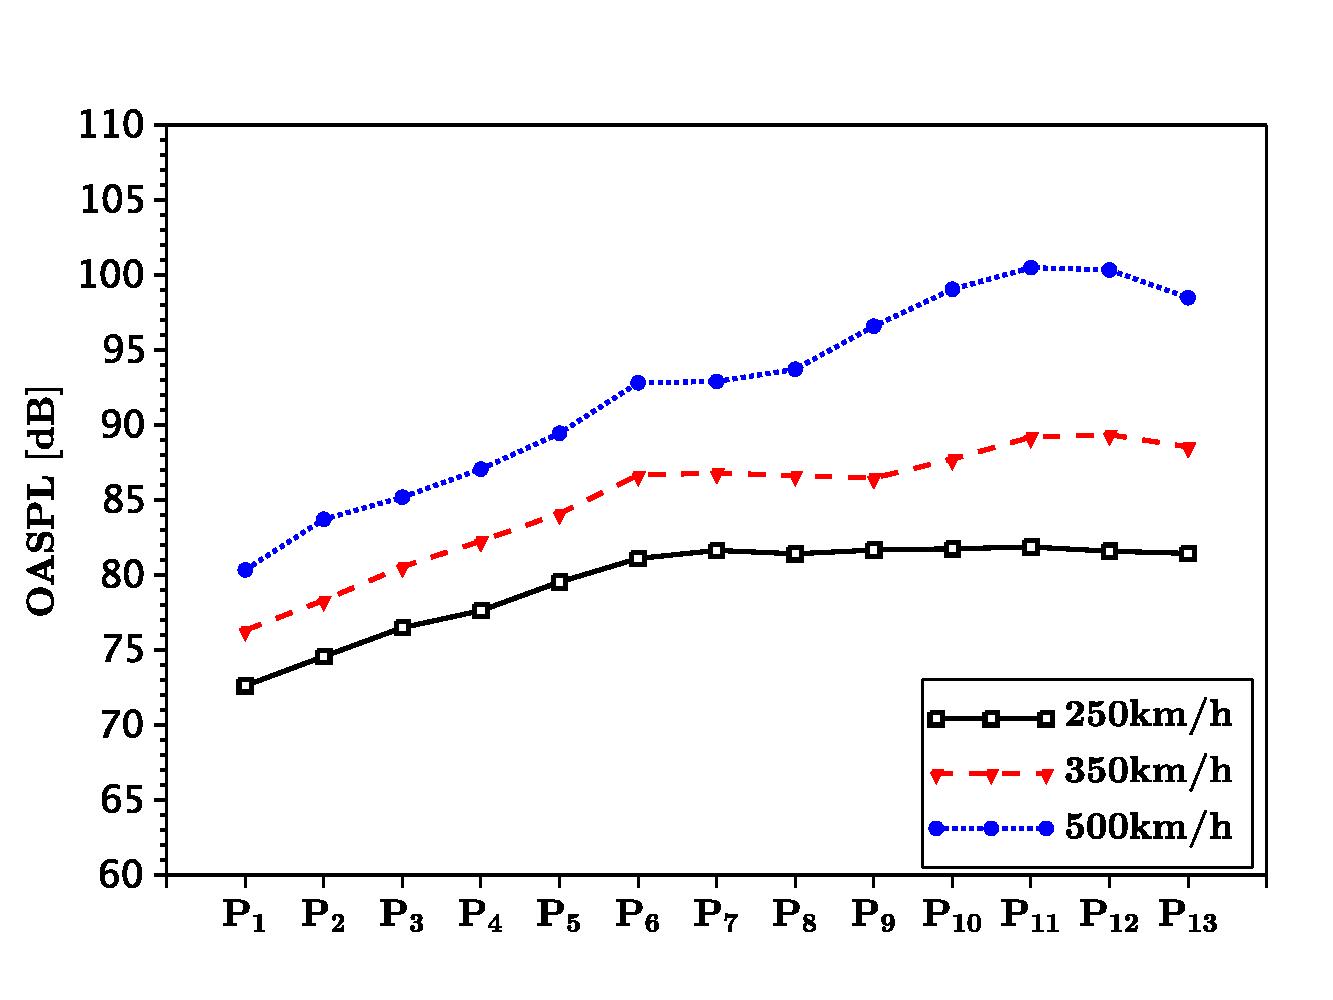
\includegraphics[width=\textwidth]{HC_OASPL_B}
    \caption{}
    \label{fig:HC_OASPL_B}
  \end{subfigure}
  \begin{subfigure}[b]{\MySubFactor\textwidth}
    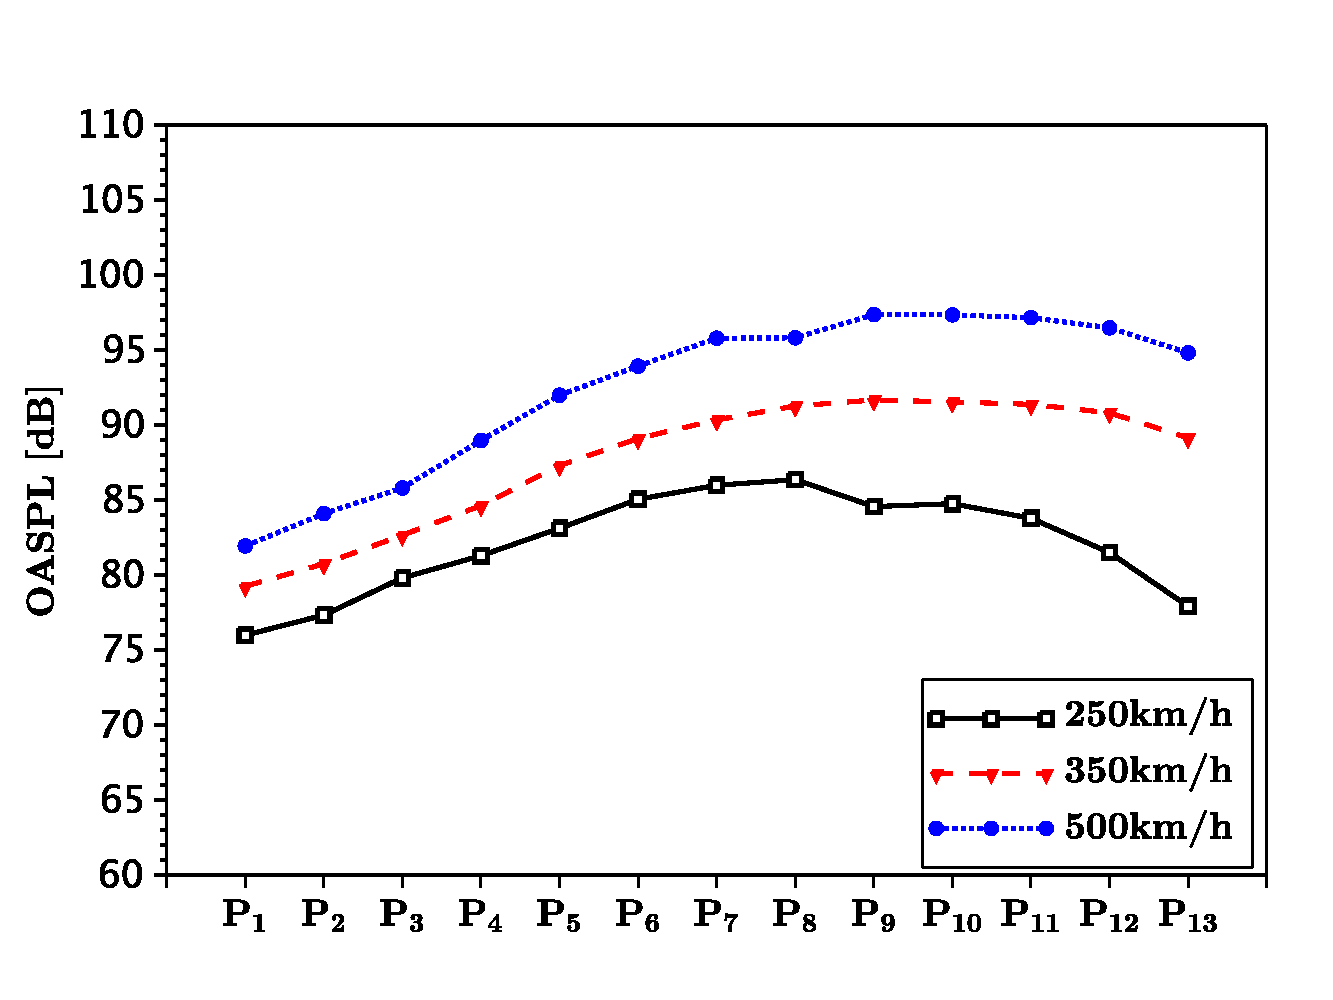
\includegraphics[width=\textwidth]{HC_OASPL_C}
    \caption{}
    \label{fig:HC_OASPL_C}
  \end{subfigure}%
  ~%add desired spacing
  \begin{subfigure}[b]{\MySubFactor\textwidth}
    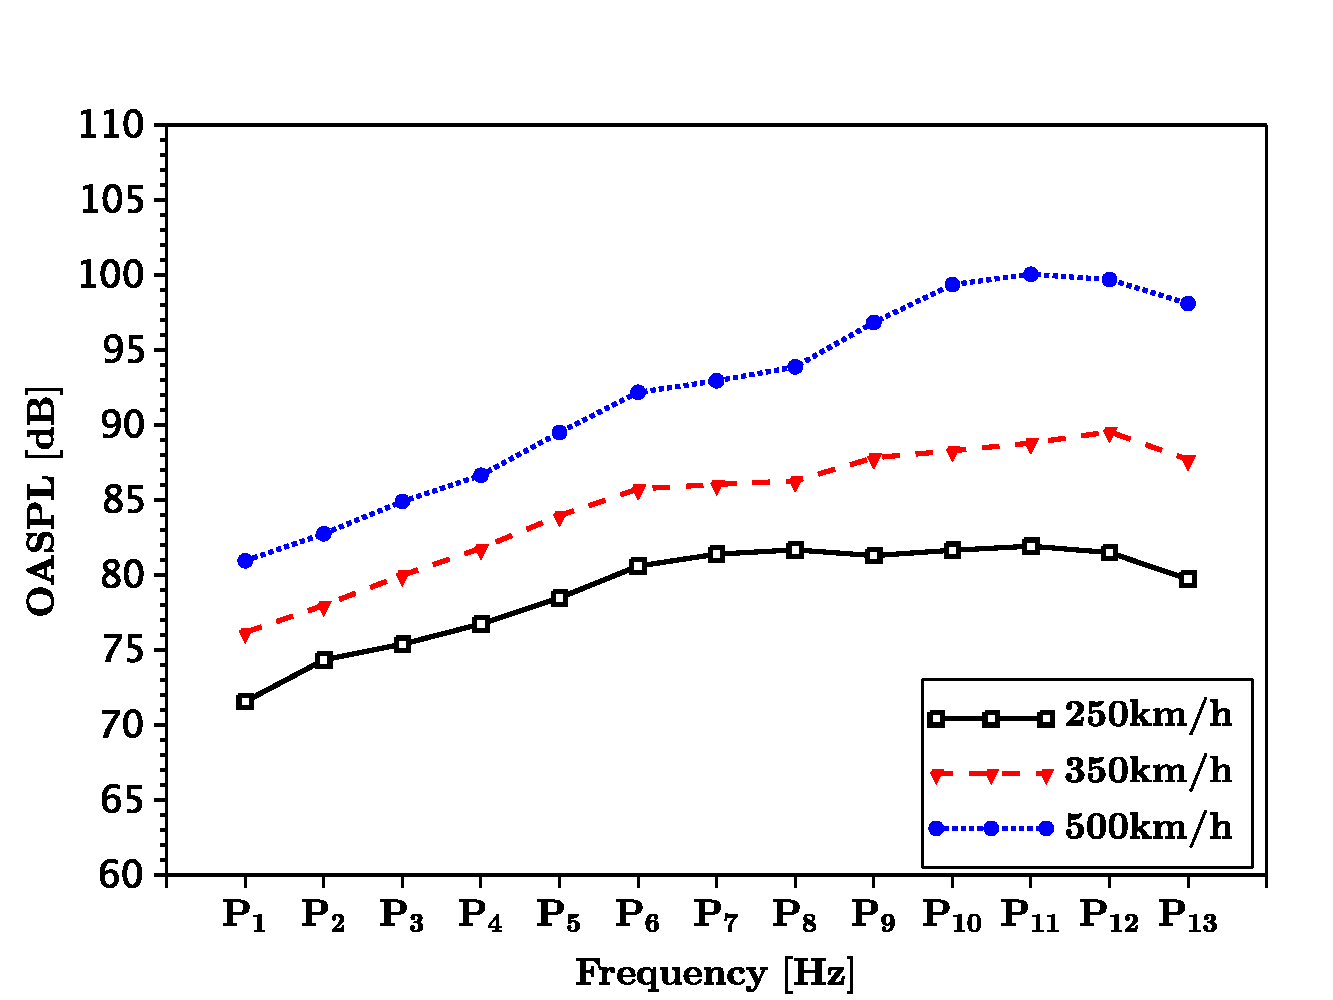
\includegraphics[width=\textwidth]{HC_OASPL_D}
    \caption{}
    \label{fig:HC_OASPL_D}
  \end{subfigure}
  \caption{总声压级。(a)$A$,(b)$B$,(c)$C$,(d)$D$}
  \label{fig:HC_OASPL}
\end{figure}
\end{verbatim}
\begin{figure}[!htbp]
  \centering
  \begin{subfigure}[b]{\MySubFactor\textwidth}
    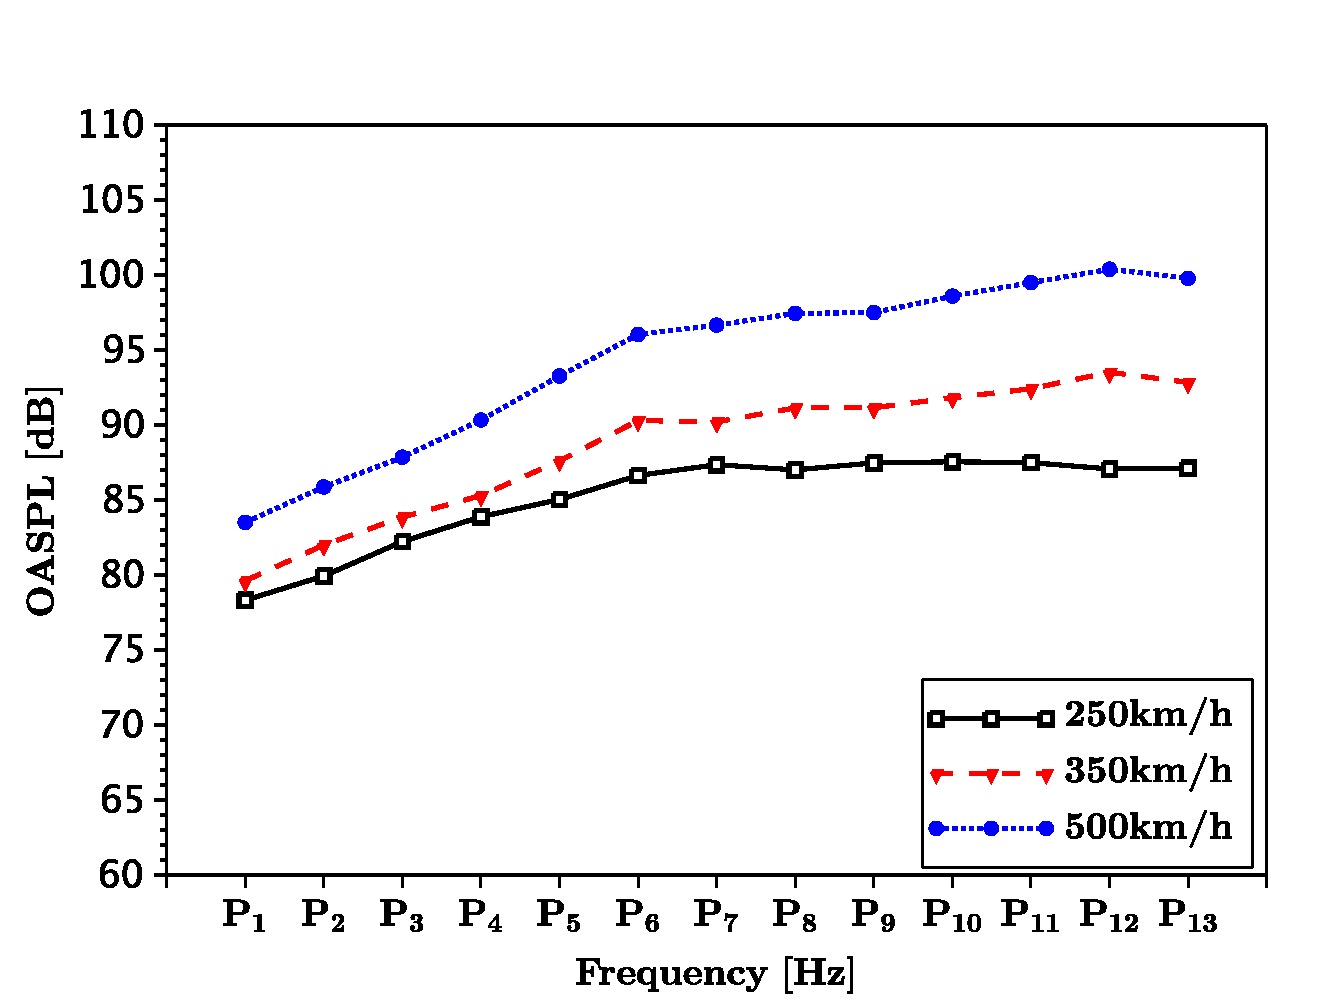
\includegraphics[width=\textwidth]{HC_OASPL_A}
    \caption{}
    \label{fig:HC_OASPL_A}
  \end{subfigure}%
  ~%add desired spacing
  \begin{subfigure}[b]{\MySubFactor\textwidth}
    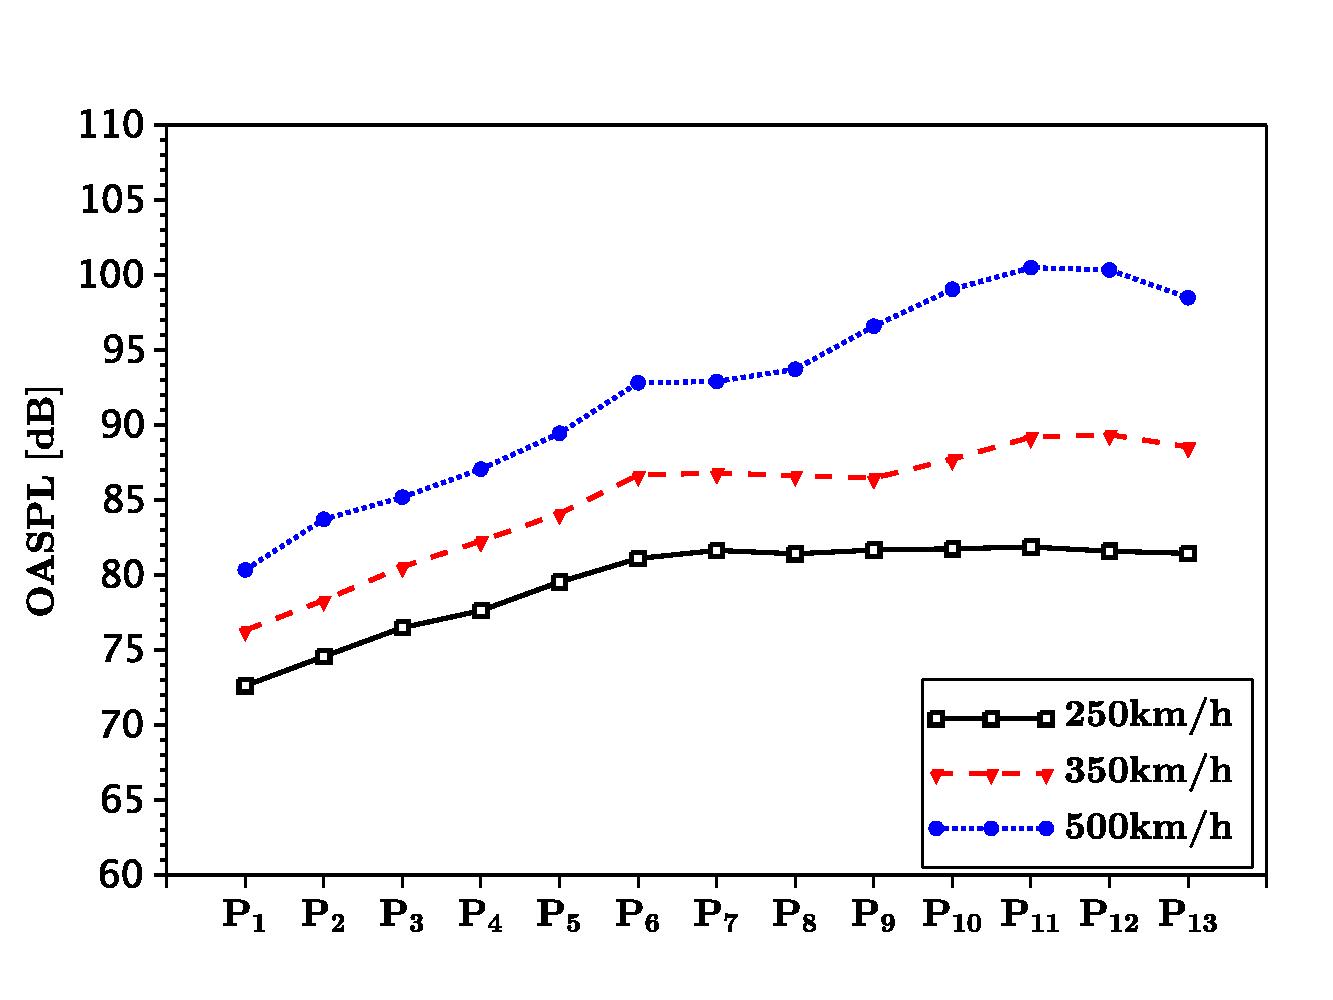
\includegraphics[width=\textwidth]{HC_OASPL_B}
    \caption{}
    \label{fig:HC_OASPL_B}
  \end{subfigure}
  \begin{subfigure}[b]{\MySubFactor\textwidth}
    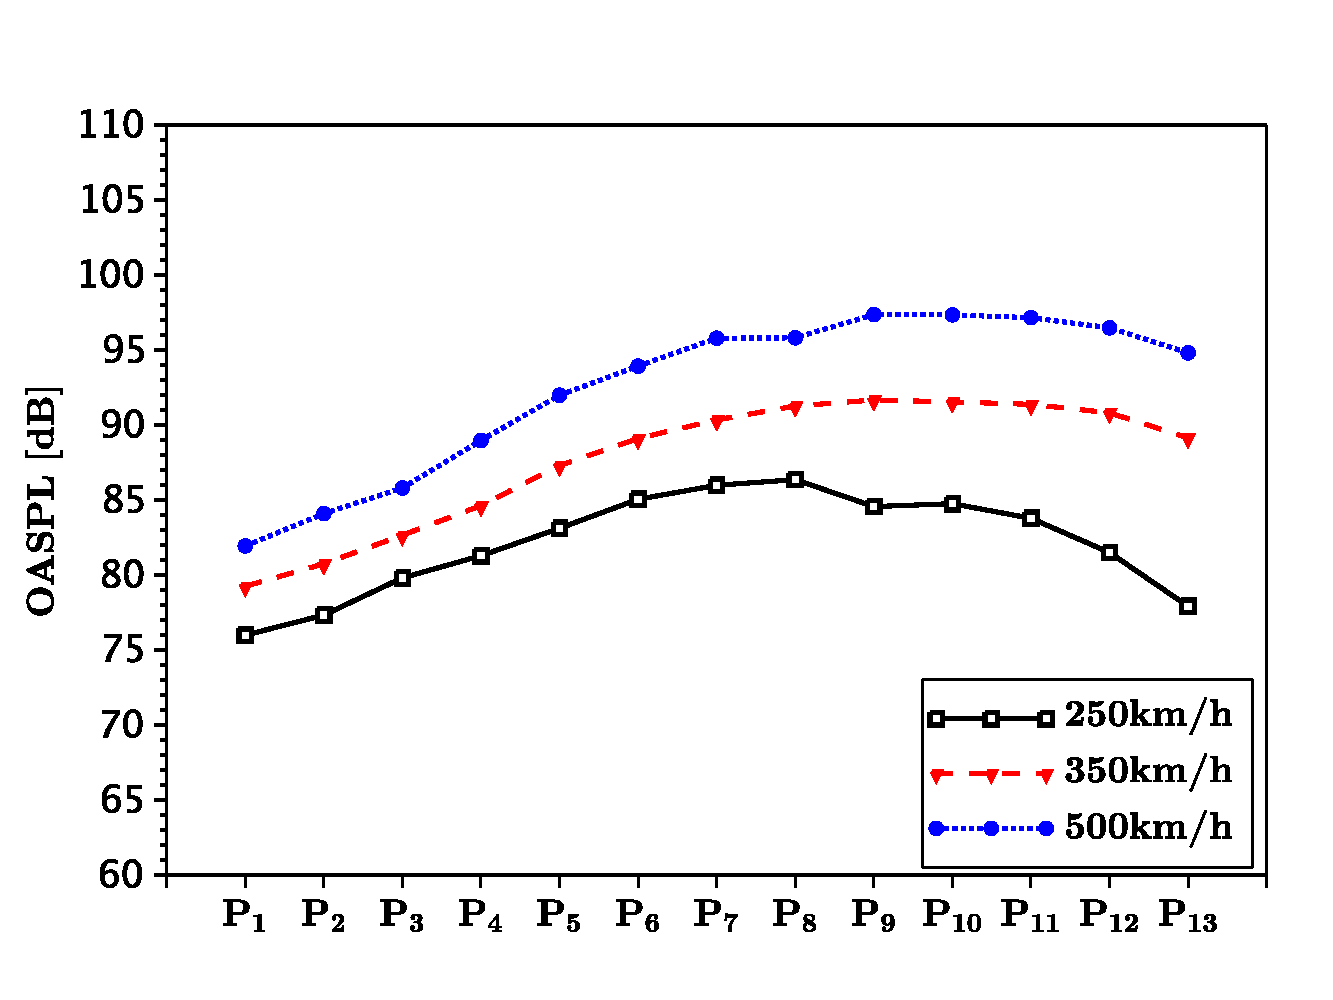
\includegraphics[width=\textwidth]{HC_OASPL_C}
    \caption{}
    \label{fig:HC_OASPL_C}
  \end{subfigure}%
  ~%add desired spacing
  \begin{subfigure}[b]{\MySubFactor\textwidth}
    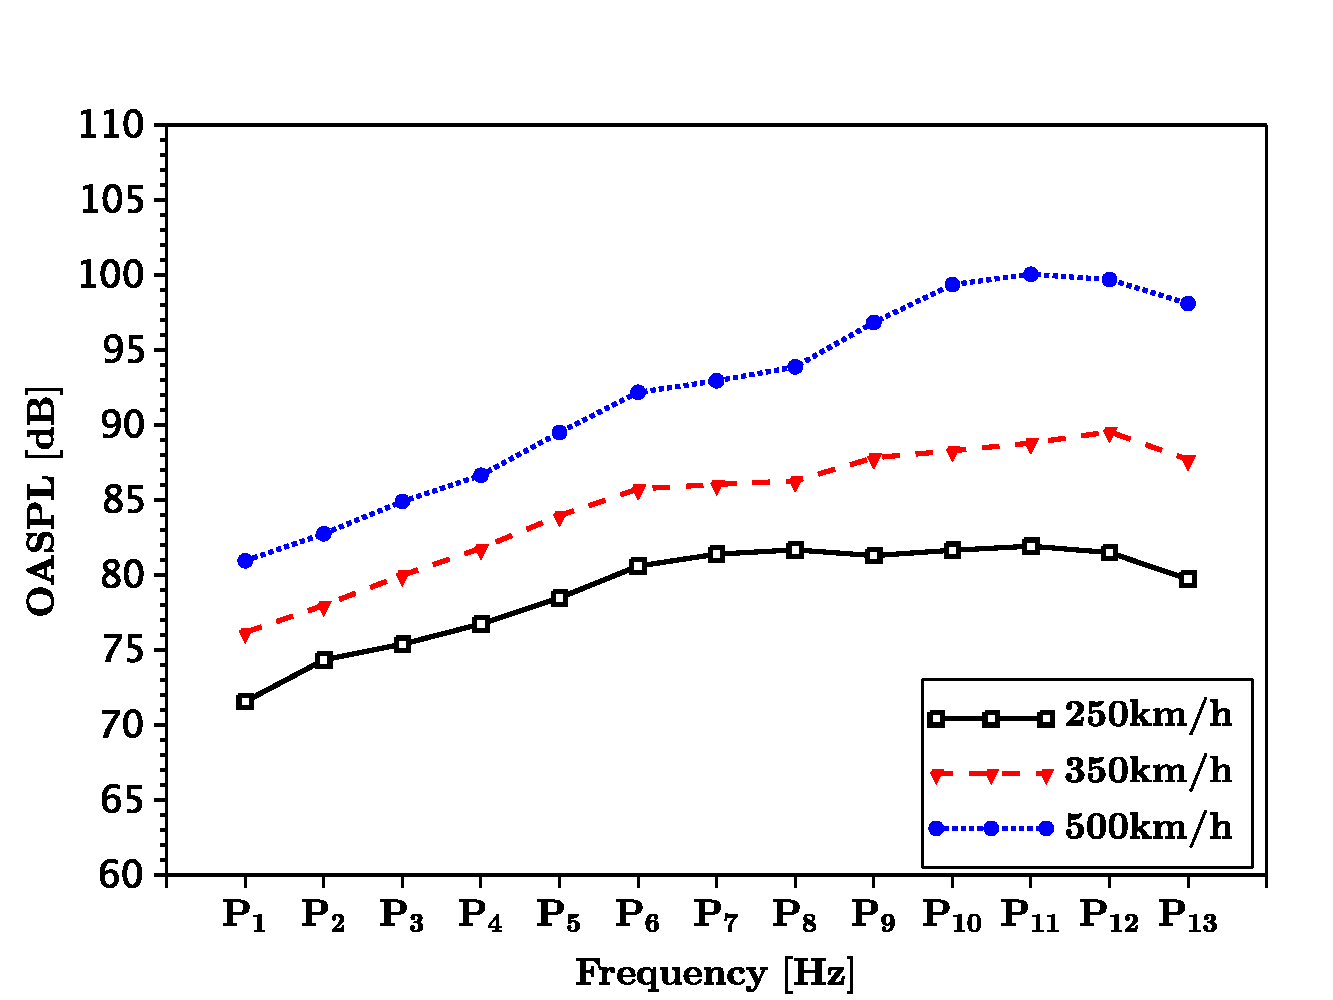
\includegraphics[width=\textwidth]{HC_OASPL_D}
    \caption{}
    \label{fig:HC_OASPL_D}
  \end{subfigure}
  \caption{总声压级。(a)$A$,(b)$B$,(c)$C$,(d)$D$}
  \label{fig:HC_OASPL}
\end{figure}

撰写论文中,插图和制表常用到的命令,已在\textbf{Useful Commands.txt}这个文本中给出了参考代码,大家只需copy使用即可。

\subsection{参考文献的使用}

参考文献的引用过程以实例的形式介绍,假设您需要引用名为“Document Preparation System”的文献,步骤如下:

1)使用“google scholar”搜索“Document Preparation System”,在目标条目下点击“引用”,展开后选择“ 导入BibTeX”,然后google将为你打开此文章的BibTeX索引信息,将它们copy添加到Myrefs.bib文件中(此文件位于“Biblio”文件夹下)。

2)你会发现索引信息中第一行为 “\verb|@article{lamport1986document,|”,其中的 
    
    "\verb|lamport1986document|" 
    
即为此文献的label,想要在论文中索引此文献,有两种索引模式:

textual mode, 输入:

“\verb|\citet{lamport1986document}|”

正如此处所示 \citet{lamport1986document}; 

parenthetical mode, 输入:

“\verb|\citep{lamport1986document}|

正如此处所示 \citep{lamport1986document}。

如此,即完成了文献的索引,请查看下本文档的“参考文献”一章,看看是不是就是这么简单呢?是的,就是这么简单!

不同的参考文献样式和文献引用样式可以通过在 "Thesis.tex" 中对 "commons.sty" 设置不同选项实现,如:

\verb+\usepackage[numbered]{commons}+ $\%$ default citation style. textual: Jones [1]; parenthetical: [1]

\verb+\usepackage[authoryear]{commons}+ $\%$ author year citation style. textual: Jones (1995); parenthetical: (Jones, 1995)

\verb+\usepackage[alpha]{commons}+ $\%$ alpha citation style. textual: not available; parenthetical: [Jon95]

参考文献索引更为详细的信息,请见\citep{wikibook2014latex}。
